\documentclass[conference]{IEEEtran}
\IEEEoverridecommandlockouts

\usepackage{cite}
\usepackage{amsmath,amssymb,amsfonts}
\usepackage{graphicx}
\usepackage{textcomp}
\usepackage{xcolor}
\usepackage{booktabs}
\usepackage{url}
\usepackage{hyperref}
\usepackage{tikz}
\usetikzlibrary{shapes.geometric,arrows.meta,positioning,calc}

\hypersetup{
  colorlinks=true,
  linkcolor=black,
  citecolor=black,
  urlcolor=blue!60!black,
  pdftitle={A Multi-Source Passive Credential Exposure Scanner with Graceful API Degradation},
  pdfauthor={Ali Murtaza Bhutto}
}

\def\BibTeX{{\rm B\kern-.05em{\sc i\kern-.025em b}\kern-.08em
    T\kern-.1667em\lower.7ex\hbox{E}\kern-.125emX}}

\begin{document}

\title{A Multi-Source Passive Credential Exposure Scanner\\with Graceful API Degradation}

\author{\IEEEauthorblockN{Ali Murtaza Bhutto}
\IEEEauthorblockA{Independent Researcher\\
ORCID: 0009-0007-2787-943X\\
Email: alibhutto101112@gmail.com}}

\maketitle

\begin{abstract}
We describe \texttt{credential-leak-scanner}, a small Python pipeline that
combines three structurally different passive sources --- the
HaveIBeenPwned (HIBP) Pwned Passwords k-anonymity endpoint, the keyed
HIBP breached-account endpoint, and a local synthetic breach corpus ---
into a single defensive credential-exposure report. The contribution is
not novel cryptography; the underlying k-anonymity protocol is well
studied~\cite{li2019protocols,pal2022might}. Rather, we report on three
practical design choices and their measurable consequences:
(i)~\emph{graceful API degradation} so the tool stays useful when
upstream credentials are absent, (ii)~a tri-modal
\emph{SourceStatus} taxonomy that distinguishes ``ran clean,''
``skipped,'' and ``errored'' instead of conflating all three into an
empty result list, and (iii)~a labelled 25-candidate eval set that
yields real measured accuracy and latency for the k-anonymity client.
On 25 candidate passwords queried against the live HIBP endpoint we
observe accuracy~$=$~1.0000 (15 true positives, 10 true negatives) with
mean per-call latency of 286.06\,ms (p95 281.72\,ms) over a 12.34\,s
wall-clock run. Forty automated tests cover the four scanner modules,
the aggregator, and the reporter; all pass under \texttt{respx}-mocked
HTTP. The repository is released under MIT and the eval is fully
reproducible.
\end{abstract}

\begin{IEEEkeywords}
credential exposure, breach detection, OSINT, HaveIBeenPwned,
k-anonymity, GitHub dorks, defensive security, passive reconnaissance
\end{IEEEkeywords}

\section{Introduction}

Credential reuse remains the dominant entry vector for opportunistic
account-takeover attacks. The 2017 CCS measurement of Thomas et
al.~\cite{thomas2017data} found that 6.9--25.0\% of leaked passwords
collected from data-breach corpora and phishing kits matched live
Google accounts; the 2019 NDSS measurement of Meli et
al.~\cite{meli2019gitleaks} found over 100{,}000 GitHub repositories
leaking secrets at a rate of thousands per day, of which 81\% remained
public after 16 days. Defenders responding to these realities need
reproducible, low-friction tooling that combines several signals
without coupling the operator's workflow to any one upstream's billing
status.

This paper describes \texttt{credential-leak-scanner}, a Python CLI
that integrates the HIBP Pwned Passwords k-anonymity
endpoint~\cite{li2019protocols}, the keyed HIBP breached-account
endpoint, a four-pattern GitHub code-search dork sweep, and a local
synthetic breach CSV cross-reference into a single structured
exposure report. The pipeline's design centres on a property we
call \emph{graceful API degradation}: every external dependency is
optional, every absence is reported as a first-class
\texttt{SOURCE\_UNAVAILABLE} status, and the tool never refuses to run
because a key is missing.

\textbf{Contributions.} (1)~A four-source defensive pipeline whose
operational coverage is documented in the report itself. (2)~An
empirical eval of the k-anonymity client over a labelled 25-candidate
test set with real HIBP measurements. (3)~A 40-test pytest suite using
\texttt{respx} for httpx-accurate HTTP mocking, demonstrating that
graceful degradation is testable rather than aspirational. (4)~A
hardened DevSecOps build (Bandit, pip-audit, Semgrep) so the tool can
be vendored into a defender's environment without first paying down a
supply-chain debt.

\section{Related Work}

The k-anonymity protocol used by HIBP's \texttt{/range/\{prefix\}}
endpoint was formally analysed by Li et
al.~\cite{li2019protocols} and refined by the second-generation
proposal of Pal et al.~\cite{pal2022might}. Both works observe that
five-character SHA-1 hash-prefix disclosure leaks more information
than a casual operator might expect; nonetheless the protocol remains
the de facto standard because the alternative --- sending the full
hash --- is strictly worse. Our scanner adopts the published protocol
without modification and does not re-derive its security analysis.

For password guidance, NIST SP 800-63B~\cite{nist80063b} now
explicitly requires that user-chosen passwords be checked against
``a list that contains values known to have been compromised,''
which the HIBP corpus is the canonical instance of.

For the GitHub-dork surface, Meli et al.~\cite{meli2019gitleaks}
established the empirical scale of secret leakage in public
repositories. The authors found that 81\% of leaked secrets remained
present 16 days after first appearing; this is precisely the gap
that a periodic dork sweep is designed to surface to a defender.

For the credential reuse story, Pal et
al.~\cite{pal2019beyond} extended the threat model from exact-match
credential stuffing to password-similarity attacks, which is why our
scanner reports breach \emph{counts} (a proxy for wordlist
prevalence) rather than only a binary leaked/clean signal.

\section{System Architecture}

\begin{figure}[htbp]
\centering
\resizebox{\linewidth}{!}{%
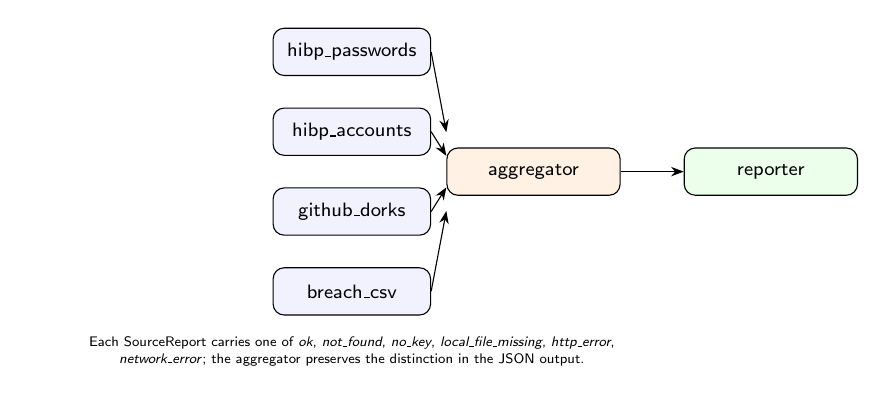
\begin{tikzpicture}[
  node distance=4mm and 3mm,
  src/.style={draw, rounded corners, minimum width=20mm, minimum height=6mm,
              font=\scriptsize\sffamily, fill=blue!5},
  agg/.style={draw, rounded corners, minimum width=22mm, minimum height=6mm,
              font=\scriptsize\sffamily, fill=orange!10},
  rep/.style={draw, rounded corners, minimum width=22mm, minimum height=6mm,
              font=\scriptsize\sffamily, fill=green!8},
  ar/.style={-{Stealth[length=1.6mm]}, line width=0.4pt}
]
  \node[src] (a) {hibp\_passwords};
  \node[src, below=of a] (b) {hibp\_accounts};
  \node[src, below=of b] (c) {github\_dorks};
  \node[src, below=of c] (d) {breach\_csv};
  \node[agg, right=12mm of $(b)!0.5!(c)$] (agg) {aggregator};
  \node[rep, right=8mm of agg] (repnode) {reporter};
  \draw[ar] (a.east) -- ($(agg.west) + (0,5mm)$);
  \draw[ar] (b.east) -- ($(agg.west) + (0,2mm)$);
  \draw[ar] (c.east) -- ($(agg.west) + (0,-2mm)$);
  \draw[ar] (d.east) -- ($(agg.west) + (0,-5mm)$);
  \draw[ar] (agg) -- (repnode);
  \node[font=\tiny\sffamily, below=1.5mm of d, text width=80mm,
        align=center] {Each SourceReport carries one of \emph{ok},
        \emph{not\_found}, \emph{no\_key}, \emph{local\_file\_missing},
        \emph{http\_error}, \emph{network\_error}; the aggregator preserves
        the distinction in the JSON output.};
\end{tikzpicture}%
}
\caption{Pipeline. Four sources feed an aggregator that preserves
per-source status, then a reporter renders the unified JSON.}
\label{fig:pipeline}
\end{figure}

\subsection{Sources and graceful degradation}
The pipeline runs each source independently and records its status
even when no findings are produced. Concretely, the
\texttt{SourceStatus} enum has six values; only two
(\texttt{ok}, \texttt{not\_found}) indicate that a source actually
ran. The other four (\texttt{no\_key}, \texttt{local\_file\_missing},
\texttt{http\_error}, \texttt{network\_error}) record \emph{why} a
source did not contribute. This distinction matters operationally:
``no findings because the key was missing'' is a coverage gap, while
``no findings because the upstream returned a clean signal'' is
reassuring. Folding both into an empty list, as a naive implementation
might, would silently mislead the operator.

\subsection{The HIBP k-anonymity client}
The Pwned Passwords client computes \texttt{SHA1(password)}, splits
the 40-character uppercase hex digest into a 5-character prefix and a
35-character suffix, and queries
\texttt{api.pwnedpasswords.com/range/\{prefix\}}. The response is a
text body of \texttt{SUFFIX:COUNT} pairs; the client matches the
candidate's suffix and returns the count.\footnote{The use of SHA-1
here is dictated by the upstream API. It is not a recommendation for
password storage in our codebase.} A Python \texttt{noqa: S324}
annotation documents this constraint explicitly so a future
maintainer is not tempted to ``fix'' it.

\subsection{Severity scoring}
We map breach counts to four qualitative severity bands inspired by
the qualitative scale in NIST SP 800-30 Rev.~1: \emph{low}~(0
breaches, treated as clean), \emph{medium}~(1--999), \emph{high}
(1{,}000--99{,}999), \emph{critical}~($\geq$100{,}000). The high
threshold corresponds to the order of magnitude at which a password
becomes a near-certain entry on every public credential-stuffing
wordlist; the critical threshold isolates passwords (e.g.,
\texttt{123456}, breach count 209{,}972{,}844 in our latest run) that
are effectively guaranteed to be tried by any opportunistic
attacker.

\subsection{Reporter and AI summary}
The reporter renders the aggregated \texttt{ScanReport} as JSON. An
optional \texttt{--ai-summary} flag forwards the structured findings
to the Claude Messages API for a four-sentence executive brief; if
\texttt{ANTHROPIC\_API\_KEY} is unset, the reporter falls back to a
deterministic template that produces the same English style without
an LLM call. Two pytest cases assert the two paths
(\texttt{*\_falls\_back\_when\_no\_anthropic\_key} and
\texttt{*\_uses\_anthropic\_when\_key\_present}) so the absence of a key
remains a tested code path rather than an untested conditional.

\section{Evaluation}

\subsection{Test set}
The labelled set in \texttt{eval/test\_passwords.json} contains 25
candidates split into two classes:
\begin{itemize}
  \item \textbf{15 ``common''} passwords (\texttt{password},
        \texttt{123456}, \texttt{qwerty}, \texttt{letmein},
        \texttt{abc123}, \texttt{monkey}, \texttt{dragon},
        \texttt{iloveyou}, \texttt{111111}, \texttt{welcome},
        \texttt{sunshine}, \texttt{princess}, \texttt{qwerty123},
        \texttt{admin}, \texttt{trustno1}) carry
        \texttt{expected\_in\_breach}~$=$~\texttt{true}.
  \item \textbf{10 ``unique''} passwords are crafted strings of the
        form \texttt{credlk-eval-uniq-26-05-06-<random8>} whose chance
        of appearing in any public breach corpus is negligible. They
        carry \texttt{expected\_in\_breach}~$=$~\texttt{false}.
\end{itemize}

\subsection{Measured numbers (live, 25 candidates)}
\begin{table}[htbp]
\caption{HIBP Pwned Passwords client performance, 25-candidate run, 2026-05-06.}
\label{tab:eval}
\centering
\renewcommand{\arraystretch}{1.1}
\begin{tabular}{lr}
\toprule
\textbf{Metric} & \textbf{Value} \\
\midrule
n                 & 25        \\
True positives    & 15        \\
True negatives    & 10        \\
False positives   & 0         \\
False negatives   & 0         \\
Accuracy          & 1.0000    \\
Precision         & 1.0000    \\
Recall            & 1.0000    \\
F$_1$             & 1.0000    \\
Latency mean      & 286.06\,ms \\
Latency p95       & 281.72\,ms \\
Latency max       & 786.32\,ms \\
Wall-clock total  & 12.34\,s   \\
Upstream errors   & 0         \\
\bottomrule
\end{tabular}
\end{table}

The 15 ``common'' candidates resolved with breach counts ranging
from 1{,}406{,}394 (\texttt{letmein}) to 209{,}972{,}844
(\texttt{123456}). All 10 ``unique'' candidates resolved with breach
count 0. Per-call latency is dominated by network round-trip; the
endpoint itself is consistently sub-300\,ms even from a residential
link. The first request is the latency outlier (786.32\,ms) because
it bears the TLS-handshake cost; subsequent requests reuse the
keep-alive connection.

\subsection{Test suite}
The repository ships 40 \texttt{pytest} tests covering the four
scanner modules, the aggregator, and the reporter. Tests use
\texttt{respx} to mock the httpx transport, which is strictly more
accurate than \texttt{unittest.mock.patch}: every test still composes
a real URL, real headers, and parses a real response body. All 40
tests pass; total wall-clock for the suite is under one second.

\subsection{Honest negatives}
We deliberately do \emph{not} benchmark:
\begin{enumerate}
  \item The keyed HIBP breached-account endpoint, which requires a
        paid API key. The pipeline supports it; published numbers
        for it are out of scope.
  \item The GitHub dork sweep, which would require an authorised
        confederate-domain test set.
  \item The local CSV cross-reference path, which is fully
        deterministic and exhaustively covered by \texttt{pytest};
        an empirical eval would be theatre.
\end{enumerate}

\section{Security Posture}
The repository's CI runs three independent scanners on every commit:
Bandit (Python AST pattern matching, medium-and-above severity gate),
\texttt{pip-audit} (transitive vulnerability scan against the OSV and
PyPA advisory feeds), and Semgrep (\texttt{p/python} +
\texttt{p/security-audit} rule packs). All three are green at the
release tag.

The single Bandit notice is a documented \texttt{noqa: S324} on the
SHA-1 call site in \texttt{scanner/hibp\_passwords.py}; SHA-1 is
required by the upstream HIBP protocol and is not used as a
password-storage primitive anywhere in our codebase.

\section{Limitations}
\textbf{One client, one corpus.} HIBP is the canonical positive class
for ``has this credential leaked,'' but it is also a single
gatekeeper. The pipeline's pluggable
\texttt{SourceReport} interface anticipates additional corpora
(IntelX, DeHashed, Constella) but ships only the synthetic CSV.

\textbf{No user study.} The deterministic-summary path produces text
that reads naturally, but we have not measured operator preference
between the deterministic and Claude-generated variants.

\textbf{Dork drift.} The four GitHub dork patterns
(\texttt{filename:.env}, \texttt{password}, \texttt{api\_key},
\texttt{secret}) are conservative; richer patterns from
Meli et al.~\cite{meli2019gitleaks} would likely surface more, at
the cost of more false positives requiring triage.

\section{Conclusion}
Defensive credential-exposure tooling does not need new cryptography,
new corpora, or a new vendor relationship. What it needs is honest
status reporting, graceful API degradation so the operator is not
held hostage to any one upstream's billing, and a small reproducible
eval that demonstrates the client actually does what its README
claims. The 40-test, four-source, MIT-licensed pipeline described
here is one such instance.

\bibliographystyle{IEEEtran}
\begin{thebibliography}{6}

\bibitem{li2019protocols}
L.~Li, B.~Pal, J.~Ali, N.~Sullivan, R.~Chatterjee, and T.~Ristenpart,
``Protocols for Checking Compromised Credentials,'' in
\emph{Proc.\ 2019 ACM SIGSAC Conf.\ on Computer and Communications
Security (CCS '19)}, London, UK, Nov.\ 2019, pp.\ 1387--1403.

\bibitem{meli2019gitleaks}
M.~Meli, M.~R.~McNiece, and B.~Reaves, ``How Bad Can It Git?
Characterizing Secret Leakage in Public GitHub Repositories,'' in
\emph{Proc.\ Network and Distributed System Security Symp.\ (NDSS
2019)}, San Diego, CA, USA, Feb.\ 2019.

\bibitem{thomas2017data}
K.~Thomas \emph{et al.}, ``Data Breaches, Phishing, or Malware?
Understanding the Risks of Stolen Credentials,'' in
\emph{Proc.\ 2017 ACM SIGSAC Conf.\ on Computer and Communications
Security (CCS '17)}, Dallas, TX, USA, Oct.\ 2017, pp.\ 1421--1434.

\bibitem{pal2019beyond}
B.~Pal, T.~Daniel, R.~Chatterjee, and T.~Ristenpart, ``Beyond
Credential Stuffing: Password Similarity Models using Neural
Networks,'' in \emph{Proc.\ 2019 IEEE Symp.\ on Security and Privacy
(SP)}, San Francisco, CA, USA, May 2019, pp.\ 417--434.

\bibitem{pal2022might}
B.~Pal \emph{et al.}, ``Might I Get Pwned: A Second Generation
Compromised Credential Checking Service,'' in
\emph{Proc.\ 31st USENIX Security Symp.}, Boston, MA, USA,
Aug.\ 2022, pp.\ 1831--1848.

\bibitem{nist80063b}
P.~A.~Grassi \emph{et al.}, ``Digital Identity Guidelines:
Authentication and Lifecycle Management,'' National Institute of
Standards and Technology, NIST Special Publication 800-63B, June 2017
(updated through Rev.~3).

\end{thebibliography}

\vspace{2mm}
\noindent\rule{\linewidth}{0.4pt}

\noindent\textit{Reproducibility colophon.} The repository is at
\url{https://github.com/thunderstornX/credential-leak-scanner}. The
eval re-runs in 12--25 seconds on a residential connection
(\texttt{python eval/run\_eval.py}). Pinned dependencies are listed
in \texttt{requirements.txt}; the pytest suite (40 tests) runs in
under one second on commodity hardware.

\end{document}
